Ein Schaltkreis wie in Abbildung \ref{fig:Abb6} dargestellt ist die Grundlage für alle Messungen. Die Als erstes müssen die Frequenzen der beiden Schwingkreise aufeinander abgestimmt werden, da eine der Kapazitäten variabel ist. \\
\begin{figure}[h!]
	\centering
	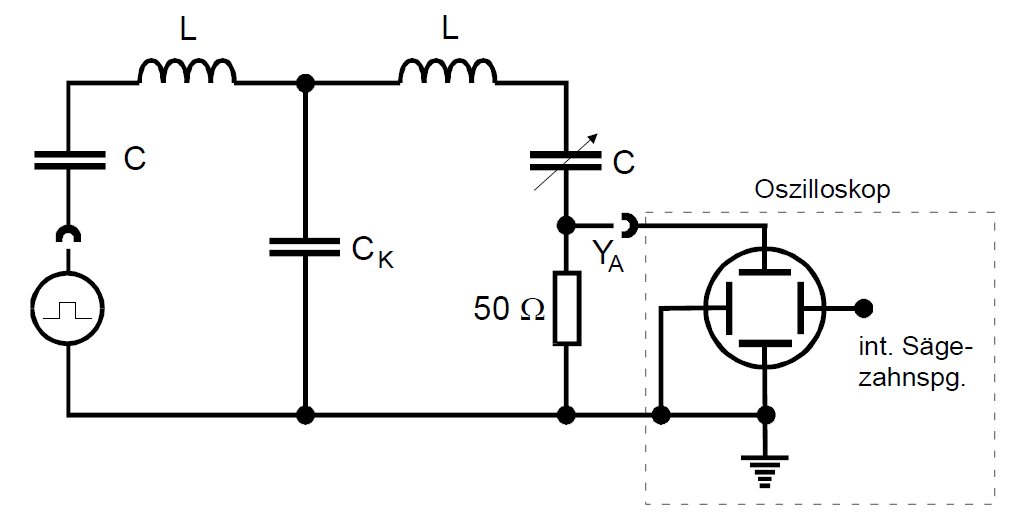
\includegraphics[width=0.5\textwidth]{Abb6.png}
	\caption{Schaltkreis für alle Messungen}
	\label{fig:Abb6}
\end{figure}
Die Frequenzen der Fundamentalschwingungen werden auf zwei Methoden bestimmt. Zuerst wird der Erreger durch eine Sinusspannung ersetzt und mit Hilfe von Lissajous-Figuren für jeden Koppelkondensator festgestellt, für welche Frequenzen bei Variation der Erregerfrequenz beide Schwingkreise um die Phasen 0 und $\pi$ verschoben sind. Bei der zweiten Methode erzeugt man ein kontinuierliches Frequenzspektrum und zeichnet den Stromverlauf des rechten Schwingkreises über die Zeit auf. Wenn der Strom ein Maximum einnimmt, ist die Frequenz gerade $\nu^+$ oder $\nu^-$. Es werden für jede Koppel-Kapazität die Zeiten am Oszilloskop abgelesen, zu denen der Strom maximal wird. \\
Des Weiteren wird die Schwebung untersucht, indem einer der beiden Schwingkreise mit einem einzelnen Impuls (bzw. Rechteckimpuls mit einer viel kleinerer Frequenz als der Schwing- und Schwegunsfrequenz) angeregt wird. Es sollen die Maxima der Schwingung innerhalb einer Schwebungsperiode für verschiedene Kapazitäten des Kondensators $C_\text{K}$ auf einem Oszilloskop beobachtet werden. Es werden also die Schwingungsmaxima (bzw. -minima) pro Schwebungsbauch gezählt.
\subsubsection*{Kenndaten der Bauteile \label{sec:Bauteile}}
Die Elemente der Schwingkreise haben die Kenngrößen
\begin{align*}
	L &= \SI{23.954}{\milli\henry} \quad\text{und} \\
	C &= \SI{0.7932}{\nano\farad} \ .
\end{align*}
Es gilt zu beachten, dass auch die Spulen eine Kapazität von
\[ C_\text{Sp} = \SI{0.028}{\nano\farad} \]
haben. Bei der späteren Berechnung der theoretischen Werte gilt daher für $\nu^+$
\[ \nu^+ = \frac{1}{2 \pi \sqrt{L(C+C_\text{Sp})}} \]
und für $\nu^-$
\[ \nu^- = \frac{1}{2 \pi \sqrt{L\left[
		\left(\frac{1}{C} + \frac{2}{C_\text{K}}\right)^{-1}+C_\text{Sp}\right]}} \ . \]